\chapter{Which capabilities should the bank build?}
\label{reading:software-conclusions}

\section{Buy a method for a question}

The software comparisons support selective reuse. A bank should first specify
the comparison it needs, then choose an estimator or discovery method whose
assumptions fit. The programming language affects maintenance and practical
use; it does not determine whether an effect is identified. Commercial support
may be worth paying for, but a licence cannot resolve an ambiguity in the
economic model. The comparisons of commercial identification, panel methods
and longitudinal inference develop this distinction in detail.

For a deposit offer, the choice begins with the population and intervention.
If the bank asks for an average effect across eligible households, an estimator
that weights households by variation in treatment answers the same question
only under additional conditions. The EconML comparison derives this issue:
a constant residual projection weights conditional effects by
$e(S)\{1-e(S)\}$, where $e(S)$ is the probability of receiving treatment in
stratum $S$. That can differ from the population average when effects vary.
This is a reason to specify and check the target, rather than to reject a
flexible estimator as a class.~\citep{exec19_econml_source,exec19_econml_reference}

Panel comparisons require the same care. In the constructed two-cohort example,
the simple treated-cell, group, dynamic and calendar averages are respectively
$4$, $19/4$, $4$ and $15/4$. The differences arise from the population and time
weights. They are not four rival estimates of an unchanged quantity. A bank
comparing suppliers should require the same target before asking which method
has narrower uncertainty or lower cost.~\citep{exec24_panelr_did,exec24_panelr_contract}

\begin{figure}[htbp]\centering
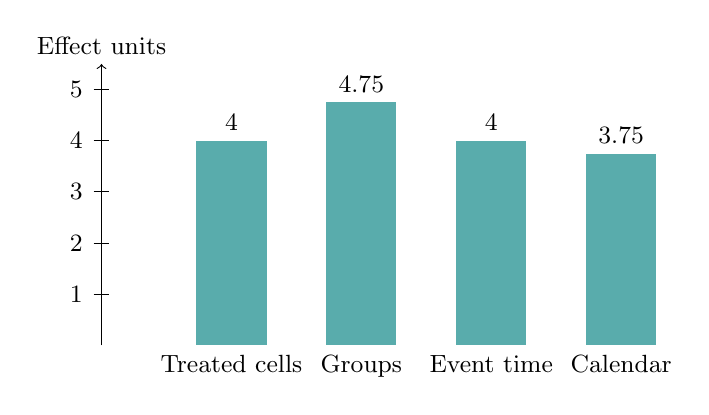
\begin{tikzpicture}[x=1.65cm,y=.65cm,every node/.style={font=\small}]
 \draw[->] (0,0)--(0,5.5) node[above]{Effect units};
 \foreach \y in {1,2,3,4,5}{\draw (-.06,\y)--(.06,\y);\node[left] at (-.07,\y){\y};}
 \foreach \x/\h in {1/4,2/4.75,3/4,4/3.75}{
  \fill[teal!65] (\x-.27,0) rectangle (\x+.27,\h);
  \node[above] at (\x,\h){\h};}
 \node[below,align=center] at (1,0){Treated\ cells};
 \node[below] at (2,0){Groups};\node[below] at (3,0){Event time};
 \node[below] at (4,0){Calendar};
\end{tikzpicture}
\caption{Different questions give different averages from the same constructed
panel. Values reproduce the two-cohort example in the R panel comparison.
They are defined averages, not empirical estimates or a ranking of packages.
\citep{exec24_panelr_contract}}
\label{reading:panel-averages}
\end{figure}

\section{A selective recommendation}

The proposal should assemble established methods around explicit economic
definitions and evidence. Rewriting every numerical method in one language
would create a second implementation to maintain and validate. Keeping an
existing implementation is preferable when it answers the required question,
can be reproduced under suitable terms, and preserves the result through the
proposed connection. Porting needs a concrete benefit, such as a deployment
constraint or a measured cost advantage, large enough to justify that extra
burden. The source comparisons establish candidate choices; the recommendation
to deploy a particular version depends on the tests described alongside it.
\citep{exec16_s10_design}

\begin{longtable}{P{.23\textwidth}P{.35\textwidth}P{.34\textwidth}}
\toprule
Banking need & Provisional choice & Evidence that could change it\\
\midrule\endhead
Effects of an offer & Reuse an estimator suited to the declared population,
adjustment variables and sampling design. Keep the financial account separate
from an arbitrary package average. & A target mismatch, poor overlap or
unreliable uncertainty in the relevant design.\\
Branch or regional rollout & Compare cohort and calendar estimands before
choosing a difference-in-differences or synthetic-control implementation. &
Unsupported comparison periods, contaminated donors or conclusions that reverse
under plausible trend departures.\\
Repeated servicing & Use a method that represents the policy's information and
the evolving observation process. & Hidden decision information, inadequate
support for the proposed actions, or poor independent policy evaluation.\\
Uncertain causal relationships & Retain the set of relationships supported by
the assumptions and data; identify effects conditional on that uncertainty. &
Credible extra knowledge or an experiment that excludes economically different
models.\\
Shared analytical service & Build the repeated work of defining questions,
reconstructing histories and interpreting comparable results; reuse numerical
methods where justified. & Evidence that ordinary analyst tools provide the
same study quality at lower full cost.\\
\bottomrule
\end{longtable}

These are proposal recommendations drawn from the preceding comparisons, not
claims that every integration has been executed. They also explain which
software details merit further investigation. A difference in coefficient
ordering is material when it changes reported uncertainty. A difference in a
random-number helper deserves priority only if it could change the statistical
conclusion or adoption choice. The conditional examples establish possible
failure mechanisms; they do not establish default-package defects or measured
coverage failures.~\citep{exec29_panel_inference_sources,exec29_panel_runtime_reference}

\section{The unresolved comparisons}

The survey remains bounded. Several commercial editions, source families and
implementation paths lack sufficiently complete primary evidence for an
unconditional comparison. Missing evidence is not evidence that a competitor
lacks a capability. The relevant question for further reading is whether a
candidate could change the proposed choice for a defined banking task.
An unresolved licence or implementation detail can defer that candidate while
other methods and other banking questions continue to be examined.

The economic conclusion is therefore selective. Start with uses for which the
bank can define the action, support the identification argument and value the
outcome. Compare the cost and reliability of reusing existing methods with the
cost of a shared service. More general ambitions remain research questions
where the necessary information or statistical result is absent.
